\section{Reconstruction from Two Views}%
\label{sec:reconstruction_two_views}


\subsection{The Reconstruction Problem}%
\label{sub:the_reconstruction_problem}


\begin{figure}[t]
	\centering
	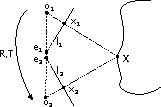
\includegraphics[width=\linewidth]{img/two-views.pdf}
	\caption{Camera motion and 3D structure from two views.}%
	\label{fig:two_views}
\end{figure}

In the last sections, we discussed how to identify point correspondences
between two consecutive frames. In this section,
we will tackle the next problem, namely that of
\textbf{reconstructing the 3D geometry of cameras and points}.
To this end, we will make the following assumptions:
\begin{itemize}
	\item We assume that we are given a
		\textbf{set of correspondences points} int two frames
		taken with the same camera from different vantage points.
	\item We assume that \textbf{the scene is static},
		i.e.\ none of the observed 3D points moved during the camera motion.
	\item We also assume that the
		\textbf{intrinsic camera (calibration) parameters are known}.
\end{itemize}

We will first estimate the \textbf{camera motion} from the set of
corresponding points. Once we know the relative location and
orientation of the cameras, we can reconstruct the 3D location
of all corresponding points by \textbf{triangulation}.\\

The projections of a point $X$ onto two images are denoted $x_1$ and $x_2$.
The optical centers of each camera are denoted by $o_1$ and $o_2$.
The intersections of the line $(o_1, o_2)$ with each image plane
are called the \textbf{epipoles} $\bm{e_1}$ and $\bm{e_2}$.
The intersections between the \textbf{epipolar plane $(\bm{o_1, o_2, X})$}
and the image planes are called \textbf{epipolar lines} $\bm{l_1}$ and $\bm{l_2}$.
There is an epipolar plane for each 3D point $X$.\\

In general 3D reconstruction is a challenging problem.
If we are given two views with 100 feature points in each of them,
then we have 200 point coordinates in 2D. The goal is to estimate
\begin{itemize}
	\item 6 parameters modeling the camera motion $R, T$
	\item $100 \times 3$ coordinates for the 3D points $X_i$
\end{itemize}
This could be done by minimizing the \textbf{projection error}:
\begin{align*}
	& E(R,T,X_1, \ldots, X_{100}) \\
	& = \sum_{j} \| x_1^j - \pi(X_j) \|^2 + \| x_2^j - \pi(R,T,X_j) \|^2
\end{align*}
This amounts to a \textbf{difficult optimization problem (not convex)} called
\textbf{bundle adjustment}. It turns out that there is a more elegant
solution which allows to entirely get rid of the 3D point coordinates.\\


\subsection{The Epipolar Constraint}%
\label{sub:the_epipolar_constraint}


We know that $x_1$ (in homogeneous coordinates) is the projection of a 3D point $X$.
Given known camera parameters ($K = 1$) and no rotation or translation
of the first camera, we merely have a projeciton with unknown depth $\lambda_1$.
From the first to the second frame we additionally have a camera
rotation and translation ($R,T$) followed by a projection.
This gives the equations:
\[
	\lambda_1 x_1 = X,
	\lambda_2 x_2 = RX + T
\]
Inserting the first equation into the second, we get:
\[
	\lambda_2 x_2 = R(\lambda_1 x_1) + T
\]
Now we remove the translation by multiplying with $\widehat{T}$:
\[
	\lambda_2 \widehat{T} x_2 = \lambda_1 \widehat{T} R x_1
\]
And projection onto $x_2$ gives the \textbf{epipolar constraint}:
\[
	\boxed{ 0 = \tr{x_2}\ \widehat{T}\ R\ x_1 }
\]
By doing all this, we have achieved to get rid of 3D coordinates.
Instead of initial constrained problem, we have a somewhat weaker,
but simpler constrained problem.
This can no longer be solved with 5 points only,
but it is much easier to solve.\\

The epipolar constraint porvides a
\textbf{relation between the 2D point coordinates} of a 3D point
in each of the two images \textbf{and the camera transformation parameters}.
The original 3D point coordinates have been removed. The matrix
\[
E = \widehat{T}R\quad \in \RR{3}{3}
\]
is called the \textbf{essential matrix}.
The \textbf{epipolar constraint} is also known as
\textbf{essential constraint} or \textbf{bilinear constraint}.
\textbf{Geometrically}, this constraint states that the three vectors
$o_1 X$, $o_2 o_1$ and $o_2 X$ form a plane, i.e.\ the triple product
of these vectors is zero.
In coordinates of the second frame, $Rx_1$ gives the direction of the
vector $o_1X$; $T$ gives the direction of $o_2 o_1$, and $x_2$
is proportional to the vector $o_2 X$ such that:
\[
	\text{volume} = \tr{x_2} (T \times Rx_1) = 0
\]

The space of all essential matrices is called the \textbf{essential space}:
\[
	\mathcal{E} \equiv \left\{ \widehat{T}R\ |\
		R \in SO(3), T \in \R^3 \right\}\ \subset \RR{3}{3}
\]
\begin{theorem}[Huang \& Faugeras, 1989 --- Characterization of the essential matrix]
	A nonzero matrix $E \in \RR{3}{3}$ is an essential matrix if and only if
	$E$ has a singular value decomposition: $(SVD)\ E = U \Sigma \tr{V}$ with
		\[
			\Sigma = \text{diag}\{ \sigma, \sigma, 0 \}
		\]
	for some $\sigma > 0$ and $U, V \in SO(3)$.
\end{theorem}
\begin{theorem}[Pose recovery from the essential matrix]
	There exists exactly two relative poses $(R,T)$ with $R \in SO(3)$
	and $T \in \R^3$ corresponding to an essential matrix $E \in \mathcal{E}$.
	For $E = U \Sigma \tr{V}$, we have:
	\begin{align*}
		(\widehat{T}_1, R_1) & =
			( U R_Z({\textstyle +\frac{\pi}{2}}) \Sigma \tr{U}
			,\ U \tr{R}_Z(+{\textstyle\frac{\pi}{2}}) \tr{V} ) \\
		(\widehat{T}_2, R_2) & =
			( U R_Z({\textstyle -\frac{\pi}{2}}) \Sigma \tr{U}
			,\ U \tr{R}_Z(-{\textstyle\frac{\pi}{2}}) \tr{V} )
	\end{align*}
	In general, only one of these gives meaningful (positive) depth.
\end{theorem}


\subsection{Eight-Point Algorithm}%
\label{sub:eight_point_algorithm}


We have seen that the 2D-coordinates of each 3D point
are coupled to the camera parameters $R$ and $T$ through an epipolar constraint.
In the following, we will derive a 3D reconstruction algorithm
which proceeds as follows:
\begin{itemize}
	\item \textbf{Recover the essential matrix $E$} from the epipolar
		constraints associated with a set of point pairs.
	\item \textbf{Extract the relative translation and rotation}
		from the essential matrix $E$.
\end{itemize}
In general, the matrix $E$ recovered from a set of epipolar constraints
will not be an essential matrix. One can resolve this problem in two ways:
\begin{enumerate}
	\item Recover some matrix $E \in \RR{3}{3}$ from the epipolar constraint
		and then project it onto the essential space.
	\item Optimize the epipolar constraints in the essential space.
\end{enumerate}
While the second approach is in principle more accurate,
it involves a nonlinear constrained optimization.
So we will pursue the first approach which is simpler and faster.\\

First we rewrite the epipolar constraint as a scalar product
in the elements of the matrix $E$ and the coordinates
of the points $x_1$ and $x_2$. Let
\[
	E^s = \tr{(e_{11}, e_{21}, e_{31}, e_{12}, e_{22}, e_{32}, e_{13}, e_{23}, e_{33})}
		\in \R^9
\]
be the vector of elements of $E$ and
\[
	a = \bm{x}_1 \otimes \bm{x}_2 \in \R^9
\]
the \textbf{Kronecker product} of the vectors $\bm{x}_i = (x_i, y_i, z_i)$.
Then the epipolar constraint can be written as:
\[
	\boxed{ \tr{\bm{x}_2} E\ \bm{x}_1 = \tr{a} E^s = 0 }
\]
For $n$ point pairs, we can combine this into the linear system:
\[
	\boxed{ \chi E^s = 0,\quad \text{with}\ \chi = \tr{(a^1, a^2, \ldots, a^n)} }
\]
We see that the vector of coefficients of the essential matrix $E$
defines the \textbf{null space of the matrix $\chi$}
In order for the above system to have a unique solution
(up to a scaling factor and ruling out the trivial solution $E = 0$),
the \textbf{rank of the matrix $\chi$ needs to be exactly 8}.
Therefore, we need at least 8 point pairs.\\

In certain \textbf{degenerate cases}, the solution for the essential matrix
is not unique even if we have 8 or more point pairs.
One such example is the case that all points lie on a line or on a plane.\\

Clearly, we will not be able to recover the sign of $E$.
Since with each $E$, there are two possible assignments of rotation $R$
and translation $T$, we therefore end up with four possible
solutions for rotation and translation.\\

The numerically estimated coefficients $E^s$ will in general fot correspond
to an essential matrix. One can resolve this problem by projecting
it back to the essential space.

\begin{theorem}[Projection onto essential space]
	Let $F \in \RR{3}{3}$ be an arbitrary matrix with SVD:
	\[
		F = U \text{diag} \{ \lambda_1, \lambda_2, \lambda_3 \} \tr{V}
		,\quad \lambda_1 \geq \lambda_2 \geq \lambda_3.
	\]
	Then the essential matrix $E$ which minimizes the Frobenius norm
	$\| F-E \|_f^2$, is given by:
	\[
		E = U \text{diag}\{ \sigma, \sigma, 0 \} \tr{V},\quad
		\text{with}\ \sigma = \frac{\lambda_1 + \lambda_2}{2}
	\]
\end{theorem}

\subsubsection*{Eight Point Algorithm (Longuet-Higgins '81) summary}%
\label{ssub:eight_point_algorithm}

Given a set of $n=8$ or more point pairs $\bm{x}_1^i, \bm{x}_2^i$:
\begin{enumerate}
	\item \textbf{Compute an approximation of the essential matrix}.
		Construct the matrix $\chi = \tr{(a^1, a^2, \ldots, a^n)}$
		where $a^i = \bm{x}_1^i \otimes \bm{x}_2^i$.
		Find the vector $E^s \in \R^9$ which minimizes $\|\chi E^s\|$
		as the ninth column of $V_{\chi}$ (smallest singular value) in the SVD
		$\chi = U_{\chi} \Sigma_{\chi} \tr{ V_{\chi} }$.
		Unstack $E^s$ into a $3 \times 3$-matrix $E$.

	\item \textbf{Project onto essential space.}
		Compute the SVD
		$E = U \text{diag} \{ \sigma_1, \sigma_2, \sigma_3 \} \tr{V}$.
		Since in the reconstruction, $E$ is only defined up to a scalar,
		we project $E$ onto the normalized essential space by replacing
		the singular values $\sigma_1, \sigma_2, \sigma_3$ with 1,1,0.

	\item \textbf{Recover the displacement from the essential matrix.}
		The four possible solutions for rotation and translation are:
		\begin{align*}
			R &= U \tr{R_Z} \left( {\textstyle \pm \frac{\pi}{2}} \right) \tr{V}, \\
			\widehat{T} &= U R_Z \left( {\textstyle \pm \frac{\pi}{2}} \right) \Sigma\ \tr{U},
		\end{align*}
		with a rotation by $\pm \frac{\pi}{2}$ around $z$:
		\[
			\tr{R_Z} \left( {\textstyle \pm \frac{\pi}{2}} \right)
				= \begin{pmatrix}
					0 & \pm 1 & 0 \\
					\mp 1 & 0 & 0 \\
					0 & 0 & 1
				\end{pmatrix}
		\]
\end{enumerate}


\subsubsection*{Do we need eight points?}%
\label{ssub:do_we_need_eight_points}


The above reasoning showed that we need at least eight points
in order for the matrix $\chi$ to have rank $8$ and therefore
guarantee a unique solution for $E$.
Yet one can take into account the special structure of $E$.
\textbf{The space of essential matrices is actually a five-dimensional space},
i.e.\ $E$ only has 5 (and not 9) degrees of freedom.\\

A simple way to \textbf{take into account the algebraic properties of $E$}
is to make use of the fact that $\det E = 0$.
If now we have only 7 point pairs, the null space of $\chi$ will have
(at least) Dimension 2, spanned by two vectors $E_1$ and $E_2$.
Then we can solve for $E$ by determining $\alpha$ such that:
\[
	\det E = \det (E_1 + \alpha E_2) = 0
\]
Along similar lines,
\textbf{Kruppa proved in 1913 that one needs only five point pairs to recover $(R,T)$.}
In the case of degenerate motion (for example planar or circular motion),
one can resolve the problem with even fewer point pairs.
Similarly, if parameters are provided by other sensors (rotation by IMU, etc.)
one can also resolve with fewer point pairs.


\subsubsection*{Limitations and Further Extensions}%
\label{ssub:limitations_and_further_extensions}


Among the four possible solutions for $R$ and $T$, there is generally
\textbf{only one meaningful one} (which assigns positive depth to all points).\\

\textbf{The algorithm fails if the translation is exactly 0},
since then $E = 0$ and nothing can be recovered.
Due to noise this typically does not happen.\\

In the case fo infinitesimal view point change, one can adapt the eight point
algorithm to the \textbf{continuous motion case}, where the epipolar constraint
is replaced by the \textbf{continuous epipolar constraint}.
Rather than recovering $(R,T)$ one recovers the linear and angular
velocity of the camera.\\

In the case of independently moving objects, one can generalize the epipolar constraint.
For two motions for example, we have either one of the other is 0:
\[
	( \tr{\bm{x}_2} E_1 \bm{x}_1 ) ( \tr{\bm{x}_2} E_2 \bm{x}_1 ) = 0
\]
with two essential matrices $E_1$ and $E_2$.
Given a sufficiently large number of point pairs, one can solve the respective
equations for multiple essential matrices using polynomial factorization.


\subsection{Structure Recontruction}%
\label{sub:structure_recontruction}


The linear eight-point algorithm allowed us to estimate the camera transformation
parameters $R$ and $T$ from a set of corresponding point pairs.
Yet, the essential matrix $E$ and hence the translation $T$ are
\textbf{only defined up to an arbitrary scale $\|E\| = \|T\| = \gamma \in \R^+$}.
After recovering $R$ and $T$, we therefore have for point $X^j$:
\[
	\lambda_2^j \bm{x}_2^j
		= \lambda_1^j R \bm{x}_1^j + \gamma T,
		\quad j = 1, \ldots, n
\]
with unknown scale parameters $\lambda_i^j$.
We can eliminate one of these scales by applying $\widehat{ \bm{x}_2^j }$:
\[
	\lambda_1^j \widehat{ \bm{x}_2^j }R \bm{x}_1^j
		+ \gamma \widehat{ \bm{x}_2^j }T
		= 0, \quad j = 1, \ldots, n
\]
This corresponds to \textbf{$n$ linear systems} of the form:
\[
	\left( \widehat{ \bm{x}_2^j }R \bm{x}_1^j
		,\ \widehat{ \bm{x}_2^j }T
	\right)
	\begin{pmatrix}
		\lambda_1^j \\ \gamma
	\end{pmatrix}
	= 0, \quad j = 1, \ldots, n
\]
Combining the parameters
$\lambda = \tr{(\lambda_1^1, \lambda_1^2, \ldots, \lambda_1^n, \gamma)} \in \R^{n+1}$,
we get the linear equation system:
\[
	\boxed{ M \lambda = 0 }
\]
with
\[
	M \equiv \left( \text{diag}(\widehat{\bm{x}_2^j} R \bm{x}_1^j)
	,\ \widehat{\bm{x}_2^j} T \right)
\]
In practice, we cannot find a solution that is exactly 0,
so we try to find $\lambda$ minimizing 
$\|M\lambda\|^2 = \tr{\lambda} \tr{M} M \lambda $ under that
$\| \lambda \| = 1$.
The linear least squares estimate for $\lambda$ is given by the eigenvector
corresponding to the smallest eigenvalue of $\tr{M}M$.
It is \textbf{only defined up to a global scale}. It reflects the
\textbf{ambiguity} that the camera has moved twice the distance,
the scene is twice larger and twice as far away.\\

This algorithm is considered \textbf{closed form} since it has an
analytic solution. But the line between analytic and numerical
solutions is often quite blurry since in practice,
eigenvalues are computed using numerical approaches at some point.


\subsection{Bundle Adjustment}%
\label{sub:bundle_adjustment}


The eight-point algorithm discussed before has several nice properties.
In particular, we found \textbf{closed-form solutions} to estimate the camera
parameters and the 3D structure, based on \textbf{singular value decomposition}.
However, if we have noisy data $\bm{\tilde{x}}_1, \bm{\tilde{x}}_2$
(correspondences not exact or even incorrect), then we have:
\begin{itemize}
	\item no guarantee that $R$ and $T$ are as close as possible
		to the true solution, some kind of robustness.
		This is mainly due to unstable eigenvalue estimation.
	\item no guarantee that we will get a consistent reconstruction.
\end{itemize}


\subsubsection*{Nonlinear Optimization Methods}%
\label{ssub:nonlinear_optimization_methods}


In order to take noise and statistical fluctuation into account,
one can revert to a \textbf{Bayesian formulation} and determine
the most likely camera transformation $R, T$ and `true'
2D coordinates $\bm{x}$ given the measured coordinates $\bm{\tilde{x}}$,
by performing a \textbf{maximum aposteriori estimate:}
\begin{align*}
	& \arg \max_{\bm{x}, R, T} \mathcal{P}(\bm{x}, R, T\ |\ \bm{\tilde{x}}) \\
	=\ & \arg \max_{\bm{x}, R, T} \mathcal{P}(\bm{\tilde{x}}\ |\ \bm{x}, R, T)
		\ \mathcal{P}(\bm{x}, R, T)
\end{align*}
This approach will however involve modeling probability densities $\mathcal{P}$
on the fairly complicated space $SO(3) \times \mathbb{S}^2$
of rotation and translation parameters, as $R \in SO(3)$ and $T \in \mathbb{S}^2$
(3D translation with unit length).\\

Alternatively, one can perform a \textbf{constrained optimization} by
minimizing a cost function (similarity to measurements):
\[
	\phi (\bm{x}, R, T) =
		\sum_{j=1}^{n} \sum_{i=1}^{2}
		\| \bm{\tilde{x}}_i^j - \bm{x}_i^j \|^2
\]
subject to (consistent geometry):
\begin{align*}
	\tr{{\bm{x}_2^j}} \widehat{T} R \bm{x}_1^j &= 0, \\
	\tr{{\bm{x}_1^j}} e_3 &= 1, \\
	\tr{{\bm{x}_2^j}} e_3 &= 1, \\
	\text{for all}\ j &= 1, \ldots, n
\end{align*}


\subsubsection*{Bundle Adjustment}%
\label{ssub:bundle_adjustment}

Interestingly, the unknown depth parameters $\lambda_i$ do not appear
in the above cost functions. The depth parameters appear directly
in the \textbf{unconstrained optimization problem}:
\[
	\sum_{j=1}^n
		\| \bm{\tilde{x}}_1^j - \pi_1 ( \bm{X}^j ) \|^2
		+ \| \bm{\tilde{x}}_2^j - \pi_2 ( \bm{X}^j ) \|^2
\]
where $\pi_i$ denote the projectinos onto the two images.
Expressed in coordinates of the first camera frame,
this is equal to the cost function:
\begin{align*}
	&\phi( \bm{x}_1, R, T, \lambda ) = \\
	&\sum_{j=1}^n
		\| \bm{\tilde{x}}_1^j - \bm{x}_1^j \|^2
		+ \| \bm{\tilde{x}}_2^j - \pi(R \lambda_1^j \bm{x}_1^j + T) \|^2
\end{align*}
This optimization procedure is known as \textbf{bundle adjustment}.
The constrained optimization and the unconstrained bundle adjustment
can be seen as
\textbf{different parameterizations of the same optimization objective}.


\subsubsection*{Degenerate Configurations}%
\label{ssub:degenerate_configurations}

The eight-point algorithm only provides unique solutions (up to a scalar factor)
if all 3D points are in a ``general position''.
This is no longer the case for certain \textbf{degenerate configurations},
for which all points lie on certain 2D surfaces which are called
\textbf{critical surfaces}.\\

Typically these critical surfaces are described by a quadratic equation
in the three point coordinates, such that they are referred to as
\textbf{quadratic surfaces}.\\

While most critical configurations do not actually arise in practice,
a specific degenerate configuration which does arise often is the case that
\textbf{all points lie on a 2D plane} (such as floors, table, walls, \ldots).\\

For the structure-from-motion problem in the context of points on a plane,
one can exploit additional constraints which leads to the so-called
\textbf{four-point algorithm}.


\subsection{Four-Point Algorithm}%
\label{sub:four_point_algorithm}


\subsubsection*{Planar Homographies}%
\label{ssub:planar_homographies}


Let us assume that all points lie on a plane. If $\bm{X}_1 \in \R^3$
denotes the point coordinates in the first frame, and these lie on a plane
with normal $N \in \mathbb{S}^2$, then we have:
\[
	\tr{N} \bm{X}_1 = d \quad \Leftrightarrow \quad
	\frac{1}{d} \tr{N} \bm{X}_1 = 1
\]
In the frame two, we therefore have the coordinates:
\begin{align*}
	\bm{X}_2
		&= R \bm{X}_1 + T \\
		&= R \bm{X}_1 + T \frac{1}{d} \tr{N} \bm{X}_1 \\
		&= \left( R + \frac{1}{d} T \tr{N} \right) \bm{X}_1 \\
		&\equiv H \bm{X}_1, \quad H \in \RR{3}{3}
\end{align*}
The matrix $H$ is called a \textbf{homography matrix}.
Inserting the 2D coordinates, we get:
\[
	\lambda_2 \bm{x}_2 = H \lambda_1 \bm{x}_1 \quad \Leftrightarrow \quad
	\boxed{ \bm{x}_2 \sim H \bm{x}_1 }
\]
Where $\sim$ means equality up to scaling.
This expression is called a \textbf{planar homography}.
$H$ depends on camera and plane parameters.


\subsubsection*{From Point Pairs to Homography}%
\label{ssub:from_point_pairs_to_homography}


By multiplying with $\widehat{\bm{x}_2}$ we can eliminate $\lambda_2$ and obtain:
\[
	\boxed{ \widehat{\bm{x}_2} H \bm{x}_1 = 0 }
\]
This equation is called the \textbf{planar epipolar constraint} or
\textbf{planar homography constraint}.
Again, we can cast this equation into the form:
\[
	\tr{\bm{a}} H^s = 0
\]
where we have stacked the elements of $H$ into a vector
\[
	H^s = (H_{11}, H_{21}, \ldots, H_{33}) \in \R^9
\]
and introduced the matrix
\[
	\bm{a} \equiv \bm{x}_1 \otimes \widehat{\bm{x}_2}\ \in \ \RR{9}{3}
\]
Since $\widehat{\bm{x}_2}$ is of rank 2, each point pair provides
two independent equations. That is why, in the general case,
we need four pairs instead of eight.


\subsubsection*{The Four Point Algorithm}%
\label{ssub:the_four_point_algorithm}

Let us now assume we have $n \geq 4$ pairs of corresponding 2D points
$\{ \bm{x}_1^j, \bm{x}_2^j \}, j= 1, \ldots, n$ in the two images.
Each point pair induces a matrix $\bm{a}^j$.
We intregrate these into a larger matrix
\[
	\chi \equiv \tr{( \bm{a}^1, \ldots, \bm{a}^n )}\ \in\ \RR{3n}{9}
\]
and obtain the system
\[
	\chi H^s = 0
\]
As in the case of the essential matrix,
\textbf{the homography matrix can be estimated up to a scale factor}.
This gives rise to the \textbf{four point algorithm}:
\begin{itemize}
	\item For the point pairs, compute the matrix $\chi$.
	\item Compute a solution $H^s$ for the above equation by singular
		value decomposition of $\chi$.
	\item Extract the motion parameters from the homography
		matrix $H = R + \frac{1}{d} T \tr{N}$.
\end{itemize}


\subsubsection*{General Comments}%
\label{ssub:general_comments}

Clearly, the derivation of the four-point algorithm is in close
analogy to that of the eight-point algorithm.\\

Rather than estimating the essential matrix $E$ on estimates the
homography matrix $H$ to derive $R$ and $T$.
In the four-point algorithm, the homography matrix is decomposed
into $R,N$ and $T/d$.
In other words, one can reconstruct the normal of the plane,
but the translation is only obtained in units of the offset $d$
of the plane and the origin.\\

The 3D structure of the points can then be computed in the same manner as before.
Since on uses the strong constraint that all points lie in a plane,
the four-point algorithm only requires four correspondences.\\

There exist numerous relations between the essential matrix $E = \widehat{T}R$
and the corresponding homography matrix $H = R + T \tr{u}$
with some $u \in \R^3$, in particular:
\[
	E = \widehat{T}H, \quad \tr{H} E + \tr{E} H = 0
\]


\subsection{The Uncalibrated Case}%
\label{sub:the_uncalibrated_case}


\subsubsection*{The Case of Uncalibrated Camera}%
\label{ssub:the_case_of_uncalibrated_camera}


The reconstruction algorithms introduced above all assume that the camera
is calibrated (K = 1). The general transformation from a 3D point to the
image is given by:
\[
	\lambda \bm{x}'\
		=\ K\, \Pi_0\, g\, \bm{X} \
		=\ (KR, KT) \bm{X}
\]
with the \textbf{intrinsic parameter matrix} or \textbf{calibration matrix}:
\[
	K = \begin{pmatrix}
		f s_x & s_{\theta} & o_x \\
		0     & f s_y & o_y \\
		0     & 0     & 1
	\end{pmatrix}
	\quad \in \RR{3}{3}
\]
The calibration matrix maps metric coordinates into image (pixel) coordinates,
using the focal length $f$, the optical center $(o_x, o_y)$,
the pixel size $(s_x, s_y)$ and a skew factor $s_{\theta}$.
If these parameters are known, then one can simply
\textbf{transform the pixel coordinates $\bm{x}'$ to normalized coordinates}
$\bm{x} = \inv{\bm{K}} \bm{x}'$
to obtain the representation used in the previous sections.
This amounts to centering the coordinates with respect to the optical center etc.


\subsubsection*{The Fundamental Matrix}%
\label{ssub:the_fundamental_matrix}

If the camera parameters $K$ cannot be estimated in a calibration procedure beforehand,
then one has to deal with \textbf{reconstruction from uncalibrated views}.\\

By transforming all image coordinates $\bm{x}'$ with the inverse calibration
matrix $\inv{K}$ into metric coordinates $x$, we obtain the
\textbf{epipolar constraint for uncalibrated cameras:}
\[
	\tr{\bm{x}_2} \widehat{T} R \bm{x}_1 = 0
	\quad \Leftrightarrow \quad
	\tr{{\bm{x'}_2}} K^{-\top} \widehat{T} R \inv{K} \bm{x'}_1 = 0
\]
which can be written as
\[
	\boxed{ \tr{{\bm{x'}_2}} F \bm{x'}_1 = 0 }
\]
with the \textbf{fundamental matrix} defined as:
\[
	F
		\quad \equiv \quad
		K^{-\top} \widehat{T} R \inv{K}
		\quad = \quad
		K^{-\top} E \inv{K}
\]
Since the invertible matrix $K$ does not affect the rank of this matrix,
we know that $F$ has an SVD $F = U \Sigma \tr{V}$ with
$\Sigma = \text{diag} ( \sigma_1, \sigma_2, 0 )$.
In fact, \textbf{any matrix of rank 2 can be a fundamental matrix}.


\subsubsection*{Limitations}%
\label{ssub:limitations}

While it is straight-forward to extend the eight-point algorithm,
such that one can extract a \textbf{fundamental matrix} from a set
of corresponding image points, it is less straight forward how to proceed from there.\\

Firstly, on cannot impose a strong constraint on the specific structure
of the fundamental matrix (apart from the fact that the last singular value is zero).\\

Secondly, for a given fundamental matrix $F$, there does not exist a finite
number of decompositions into extrinsic parameters $R,T$ and intrinsic
parameters $K$ (even apart from the global scale factor).\\

As a consequence, one can only determine so-called \textbf{projective reconstructions}
i.e.\ reconstructions of geometry and camera position which are defined
up to a so-called projective transformation.\\

As a solution, one typically choses a \textbf{canonical reconstruction}
from the family of possible reconstructions.
